% LipScribe -- From Cole: To the Rest (Complete Project Handbook, Weeks 1 to 4)
% Compile: tectonic from_cole_to_the_rest.tex  (or pdflatex from_cole_to_the_rest.tex)
\documentclass[11pt,a4paper]{article}
\usepackage{lipscribe-report}
\usepackage{graphicx}
\usepackage{amsmath}
\usepackage{float}
\usepackage{tikz}
\usepackage{listings}
\usetikzlibrary{arrows.meta,positioning,shapes.geometric}

\fancyhead[L]{\small\sffamily\color{lsgrey}From Cole: To the Rest -- Complete LipScribe Technical Handbook (Weeks 1--4)}

\definecolor{codebg}{RGB}{246,248,250}
\definecolor{codeframe}{RGB}{208,215,222}
\definecolor{codecomment}{RGB}{87,96,106}
\definecolor{codekw}{RGB}{15,76,129}

\lstset{
  basicstyle=\ttfamily\footnotesize,
  backgroundcolor=\color{codebg},
  frame=single,
  rulecolor=\color{codeframe},
  framesep=5pt,
  xleftmargin=6pt,
  xrightmargin=6pt,
  breaklines=true,
  breakatwhitespace=true,
  columns=fullflexible,
  keepspaces=true,
  commentstyle=\color{codecomment}\itshape,
  keywordstyle=\color{codekw}\bfseries,
  showstringspaces=false,
  upquote=true
}

\newcommand{\code}[1]{\texttt{\small #1}}
\newcommand{\tile}[2]{\colorbox{lslight}{\parbox[t][1.55cm][t]{0.212\textwidth}{\sffamily\raggedright
  {\Large\bfseries\color{lsblue}#1}\par\vspace{3pt}{\scriptsize\linespread{1.0}\selectfont #2\par}}}}
\newcommand{\callout}[2]{%
  \par\smallskip\noindent
  \colorbox{lslight!65}{\parbox{\dimexpr\textwidth-2\fboxsep\relax}{%
    \vspace{3pt}{\sffamily\bfseries\color{lsblue}#1}\par\vspace{2pt}{\small #2}\vspace{3pt}}}%
  \par\smallskip
}

\newcolumntype{L}[1]{>{\raggedright\arraybackslash}p{#1}}
\setlength{\textfloatsep}{10pt plus 2pt minus 2pt}
\setlength{\floatsep}{8pt plus 2pt minus 2pt}
\setlist{itemsep=2pt,topsep=3pt,parsep=0pt}

\begin{document}

\docheader{From Cole: To the Rest}{The Complete LipScribe Technical Handbook: Everything Achieved, Every Setback Met, and Every Decision Taken (Weeks 1--4)}{9 November 2026}

\callout{A Note from Cole to Charis, Faith, Lisa, Nehum, and Isabelle}{%
This booklet is written as a complete, self-contained tutor guide so that every member of Group~4 has the exact same deep understanding of our entire system---from raw video and audio files in Week~1 all the way to our state-of-the-art \textbf{Proposed Model~P} in Week~4. Nothing is skipped: every mathematical intuition, every bug and setback we hit, why it happened, how we fixed it, every graph, and every terminal command you need to run the codebase yourself is right here.}

\medskip
\noindent\tile{32,890}{Verified GRID clips across 33 speakers (96.7\,\% pass rate)}\hfill%
\tile{1.02\,\%}{Best greedy clean test WER (Model P4; 0.71\,\% with grammar)}\hfill%
\tile{1.88\,\%}{Model P4 no-video fallback WER (vs.\ 25.18\,\% for B3 v2)}\hfill%
\tile{30.9\,\%}{Visual lip gate weight at $-$5\,dB (up from 19.6\,\% clean)}

\tableofcontents
\vspace{6pt}
{\color{lsblue}\rule{\textwidth}{0.5pt}}

% =====================================================================
\section{Chapter 1 --- The Big Picture: What Problem Are We Solving (and How CTC Works)?}

\subsection{Why Audio-Only Recognition Fails in Noise and Why Lips Alone Are Not Enough}
When someone speaks in a quiet room (\textbf{Clean} condition), an audio-only speech recogniser easily separates vowels and consonants from the spectrogram. However, as background noise increases---measured as \textbf{Signal-to-Noise Ratio (SNR)} dropping from $\text{Clean} \to 10\,\text{dB} \to 5\,\text{dB} \to 0\,\text{dB} \to -5\,\text{dB}$ (where $-5\,\text{dB}$ means background noise power is \textbf{3.16$\times$ stronger} than the voice!)---acoustic formants and high-frequency consonant bursts (\code{/f/}, \code{/s/}, \code{/b/}, \code{/p/}) are buried.

\textbf{Visual lip movements are 100\,\% immune to acoustic noise}: whether the room is silent or at $-5\,\text{dB}$, the mouth pixels are identical. Conversely, lipreading alone struggles with \textbf{homophenes}---distinct sounds produced with virtually identical lip shapes (e.g., bilabials \code{/b/}, \code{/p/}, \code{/m/} or alveolars \code{/d/}, \code{/t/}, \code{/n/}). Therefore:
\begin{itemize}
  \item \textbf{Audio} provides voicing and nasality (separating \code{/b/} from \code{/p/} and \code{/m/}).
  \item \textbf{Video (Lips)} provides place of articulation and lip aperture (separating \code{/b/} from \code{/f/} or \code{/s/} even when noise drowns the microphone).
\end{itemize}

\subsection{The 75-Frame Temporal Synchronisation Contract ($3.0\,\text{s} = 75\text{ Frames}$)}
Every clip in the GRID corpus lasts $3.0\text{ seconds}$ at $25\text{ frames per second (fps)}$, giving $T = 75$ video frames (one frame every $40\,\text{ms}$):
\begin{itemize}
  \item \textbf{Video stream:} $25\text{ fps} \times 3.0\text{ s} = 75$ grayscale mouth frames of size $96 \times 96 \implies [B, 1, 75, 96, 96]$.
  \item \textbf{Audio stream:} $16{,}000\text{ Hz}$ waveform ($48{,}000$ samples) converted to 80-band log-Mel spectrograms using a $25\,\text{ms}$ Hann window and $10\,\text{ms}$ hop ($100\text{ frames/s}$) $\implies [B, 300, 80]$.
  \item \textbf{Exact $4:1$ alignment:} Notice that $300 \div 4 = 75$. In \code{lipscribe/models/audio\_encoder.py}, two \code{Conv1d} layers each with $\text{stride}=2$ downsample time by $2 \times 2 = 4$ ($[B, 300, 80] \to [B, 150, 256] \to [B, 75, 256]$), followed by a 2-layer BiLSTM outputting $[B, 75, 512]$.
  \item Meanwhile, our visual encoder (\code{VisualEncoder} or \code{ResNetVisualEncoder}) uses temporal stride $1$, outputting $[B, 75, 512]$. Thus at every frame index $t \in \{1,\dots,75\}$, the audio vector $\mathbf{a}_t \in \mathbb{R}^{512}$ and visual vector $\mathbf{v}_t \in \mathbb{R}^{512}$ describe the \textbf{exact same $40\,\text{ms}$ slice of speech}.
\end{itemize}

\begin{figure}[H]
\centering
\resizebox{\textwidth}{!}{%
\begin{tikzpicture}[
  box/.style={draw=lsblue, fill=lslight!60, rounded corners=3pt, align=center, font=\sffamily\scriptsize, minimum height=0.88cm, inner sep=3pt, line width=0.6pt},
  fbox/.style={draw=lsdone, fill=lsdone!12, rounded corners=3pt, align=center, font=\sffamily\scriptsize, minimum height=0.88cm, inner sep=3pt, line width=0.7pt},
  arr/.style={-{Stealth[length=4pt]}, lsblue, line width=0.7pt}
]
  \node[box, text width=2.9cm] (v) at (0, 0.8) {\textbf{Mouth Video}\\$[B, 1, 75, 96, 96]$\\(25 fps)};
  \node[box, text width=2.9cm] (a) at (0, -0.8) {\textbf{Log-Mel Audio}\\$[B, 300, 80]$\\(100 fps)};

  \node[box, text width=3.3cm] (ve) at (3.9, 0.8) {\textbf{Visual Encoder (V1 / V2)}\\Temporal stride $= 1$\\$\to \mathbf{v}_t \in [B, 75, 512]$};
  \node[box, text width=3.3cm] (ae) at (3.9, -0.8) {\textbf{Audio Encoder}\\$2\times$ Stride-2 \code{Conv1d} + BiLSTM\\$\to \mathbf{a}_t \in [B, 75, 512]$};

  \node[fbox, text width=3.6cm] (fu) at (8.2, 0) {\textbf{Multimodal Fusion}\\B3 Concat \emph{or} Model P\\($\mathbf{e}_{\text{miss}}$ + Cross-Attn + Gate $\mathbf{g}_t$)\\$\to \mathbf{f}_t \in [B, 75, 256]$};

  \node[box, text width=3.2cm] (ctc) at (12.3, 0) {\textbf{CTC Sequence Head}\\BiLSTM + Linear($256{\to}28$)\\Log-Probs $[75, B, 28]$\\$\to$ Greedy / Beam / Grammar};

  \draw[arr] (v) -- (ve);
  \draw[arr] (a) -- (ae);
  \draw[arr] (ve.east) -- (fu.west);
  \draw[arr] (ae.east) -- (fu.west);
  \draw[arr] (fu) -- (ctc);
\end{tikzpicture}%
}
\caption{End-to-end LipScribe tensor flow and the $75$-frame ($25\,\text{fps}$) alignment contract fixed in \code{docs/INTERFACES.md}.}
\label{fig:arch_overview}
\end{figure}

\subsection{How CTC (Connectionist Temporal Classification) Works}
We have $T = 75$ frames, whereas a target transcript like \code{"bin blue at f two now"} has only $L = 21$ characters, and we do not know which exact frame corresponds to each letter. \textbf{CTC} solves alignment-free sequence learning by adding a special \code{<blank>} symbol (index \code{0}) to our character vocabulary (\code{space = 1}, \code{a..z = 2..27}), giving \textbf{28 classes}:
\begin{enumerate}
  \item \textbf{Step 1 (Merge consecutive duplicates):} \code{[b, b, 0, i, i, n, 0, n]} $\to$ \code{[b, 0, i, n, 0, n]}.
  \item \textbf{Step 2 (Remove all blanks \code{0}):} \code{[b, 0, i, n, 0, n]} $\to$ \code{"binn"}.
  \item \textbf{Why blank is required for double letters:} In words like \code{"green"} or \code{"soon"}, emitting \code{[e, e]} collapses to a single \code{"e"}. To output \code{"ee"}, the network \emph{must} emit \code{[e, 0, e]}. Consequently, a transcript of length $L$ with $R$ repeated adjacent characters requires at least $L + R$ frames. Across all 33,000 GRID transcripts, the longest sentence is $31$ characters with at most $3$ adjacent repeats ($31 + 3 = 34 \le 75$), so $T=75$ never violates the CTC length condition.
\end{enumerate}

% =====================================================================
\section{Chapter 2 --- Week 1: Data Integrity, End-Pointed Audio, Speaker Splits, and Mouth Cropping}

\subsection{Setbacks \#1 \& \#2: What \code{verify\_dataset.py} Uncovered in the Raw GRID Corpus}
Before training anything, Faith wrote \code{scripts/verify\_dataset.py} (Card \textbf{W1-07}) to audit all 34,000 raw GRID utterances across 7 checks. This immediately caught two major data traps:
\begin{itemize}
  \item \textbf{Setback \#1 (Missing Speaker \code{s21} \& Corrupted Clips):} Speaker \code{s21} had audio files only (zero videos or alignments); speaker \code{s8} had $108$ undecodable videos; \code{s4} had $1$ bad video (\code{bbbm2n}); \code{s28} had $1$ bad audio clip. \textbf{Decision:} Excluded \code{s21} and filtered out the 110 corrupted clips, leaving \textbf{32,890 verified utterances across 33 speakers (96.7\,\% pass rate)}.
  \item \textbf{Setback \#2 (End-Pointed Audio Desynchronisation):} While every video lasted $3.0\,\text{s}$ ($75$ frames), the raw GRID \code{.wav} files were \emph{end-pointed} (trimmed to only the spoken portion, lasting $1.10\text{--}2.94\,\text{s}$, mean $1.83\,\text{s}$), whereas speakers sat silently for an average of $0.47\,\text{s}$ (up to $1.51\,\text{s}$) into the video before speaking! If we placed the audio at $t = 0$, the voice would play $0.5\text{--}1.5\,\text{s}$ \textbf{ahead of the lips}. \textbf{Decision:} In \code{lipscribe/data/dataset.py}, we read the exact word-onset timestamp from each utterance's \code{.align} file and shift the audio waveform into a $3.0\,\text{s}$ ($48{,}000$-sample) buffer at the exact frame the lips begin moving.
\end{itemize}

\subsection{Speaker-Independent Splits (\code{splits.csv}) \& Disjoint MUSAN Noise Pools (\code{noise\_splits.csv})}
To guarantee zero speaker or noise leakage:
\begin{itemize}
  \item \textbf{Speaker split (\code{data/splits.csv}, seed 2026):} \textbf{Train}: 26 speakers (14M, 12F; $25{,}891$ clips). \textbf{Validation}: 3 unseen speakers (\code{s11}, \code{s19}, \code{s26}; $3{,}000$ clips). \textbf{Test}: 4 unseen speakers (\code{s4}, \code{s9}, \code{s14}, \code{s24}; 2M, 2F; $3{,}998$ usable clips).
  \item \textbf{MUSAN noise split (\code{data/noise\_splits.csv}):} Split \emph{by noise file} (70\,\% train / 15\,\% val / 15\,\% test) so test noise files are never heard during training.
\end{itemize}

\subsection{Setback \#3: MediaPipe Mouth-Cropping Failure Handling (\code{lipscribe/preprocessing/crop.py})}
In Cards \textbf{W1-10} and \textbf{W2-01}, I built the mouth-cropping pipeline using MediaPipe Face Mesh (\code{FACEMESH\_LIPS} landmarks, square bounding box $+25\,\%$ margin, smoothed with a centred 5-frame moving average, resized to $96{\times}96$ grayscale \code{uint8}).
\begin{itemize}
  \item \textbf{Setback \#3 (What if Face Mesh misses a frame?):} If MediaPipe fails on 1--2 frames and we drop those frames, $T$ shrinks from $75$ to $73$ and breaks audio--video alignment.
  \item \textbf{Decision:} \textbf{Never drop frames.} Failed frames linearly interpolate their crop bounding box from the nearest valid frames before and after, while recording \code{valid[t] = False} in the per-frame validity mask (Figure~\ref{fig:crops_handbook}). Clips with $> 10\,\%$ invalid frames are excluded in \code{build\_manifest.py}.
\end{itemize}

\begin{figure}[H]
\centering
\begin{minipage}[t]{0.33\textwidth}\vspace{0pt}
  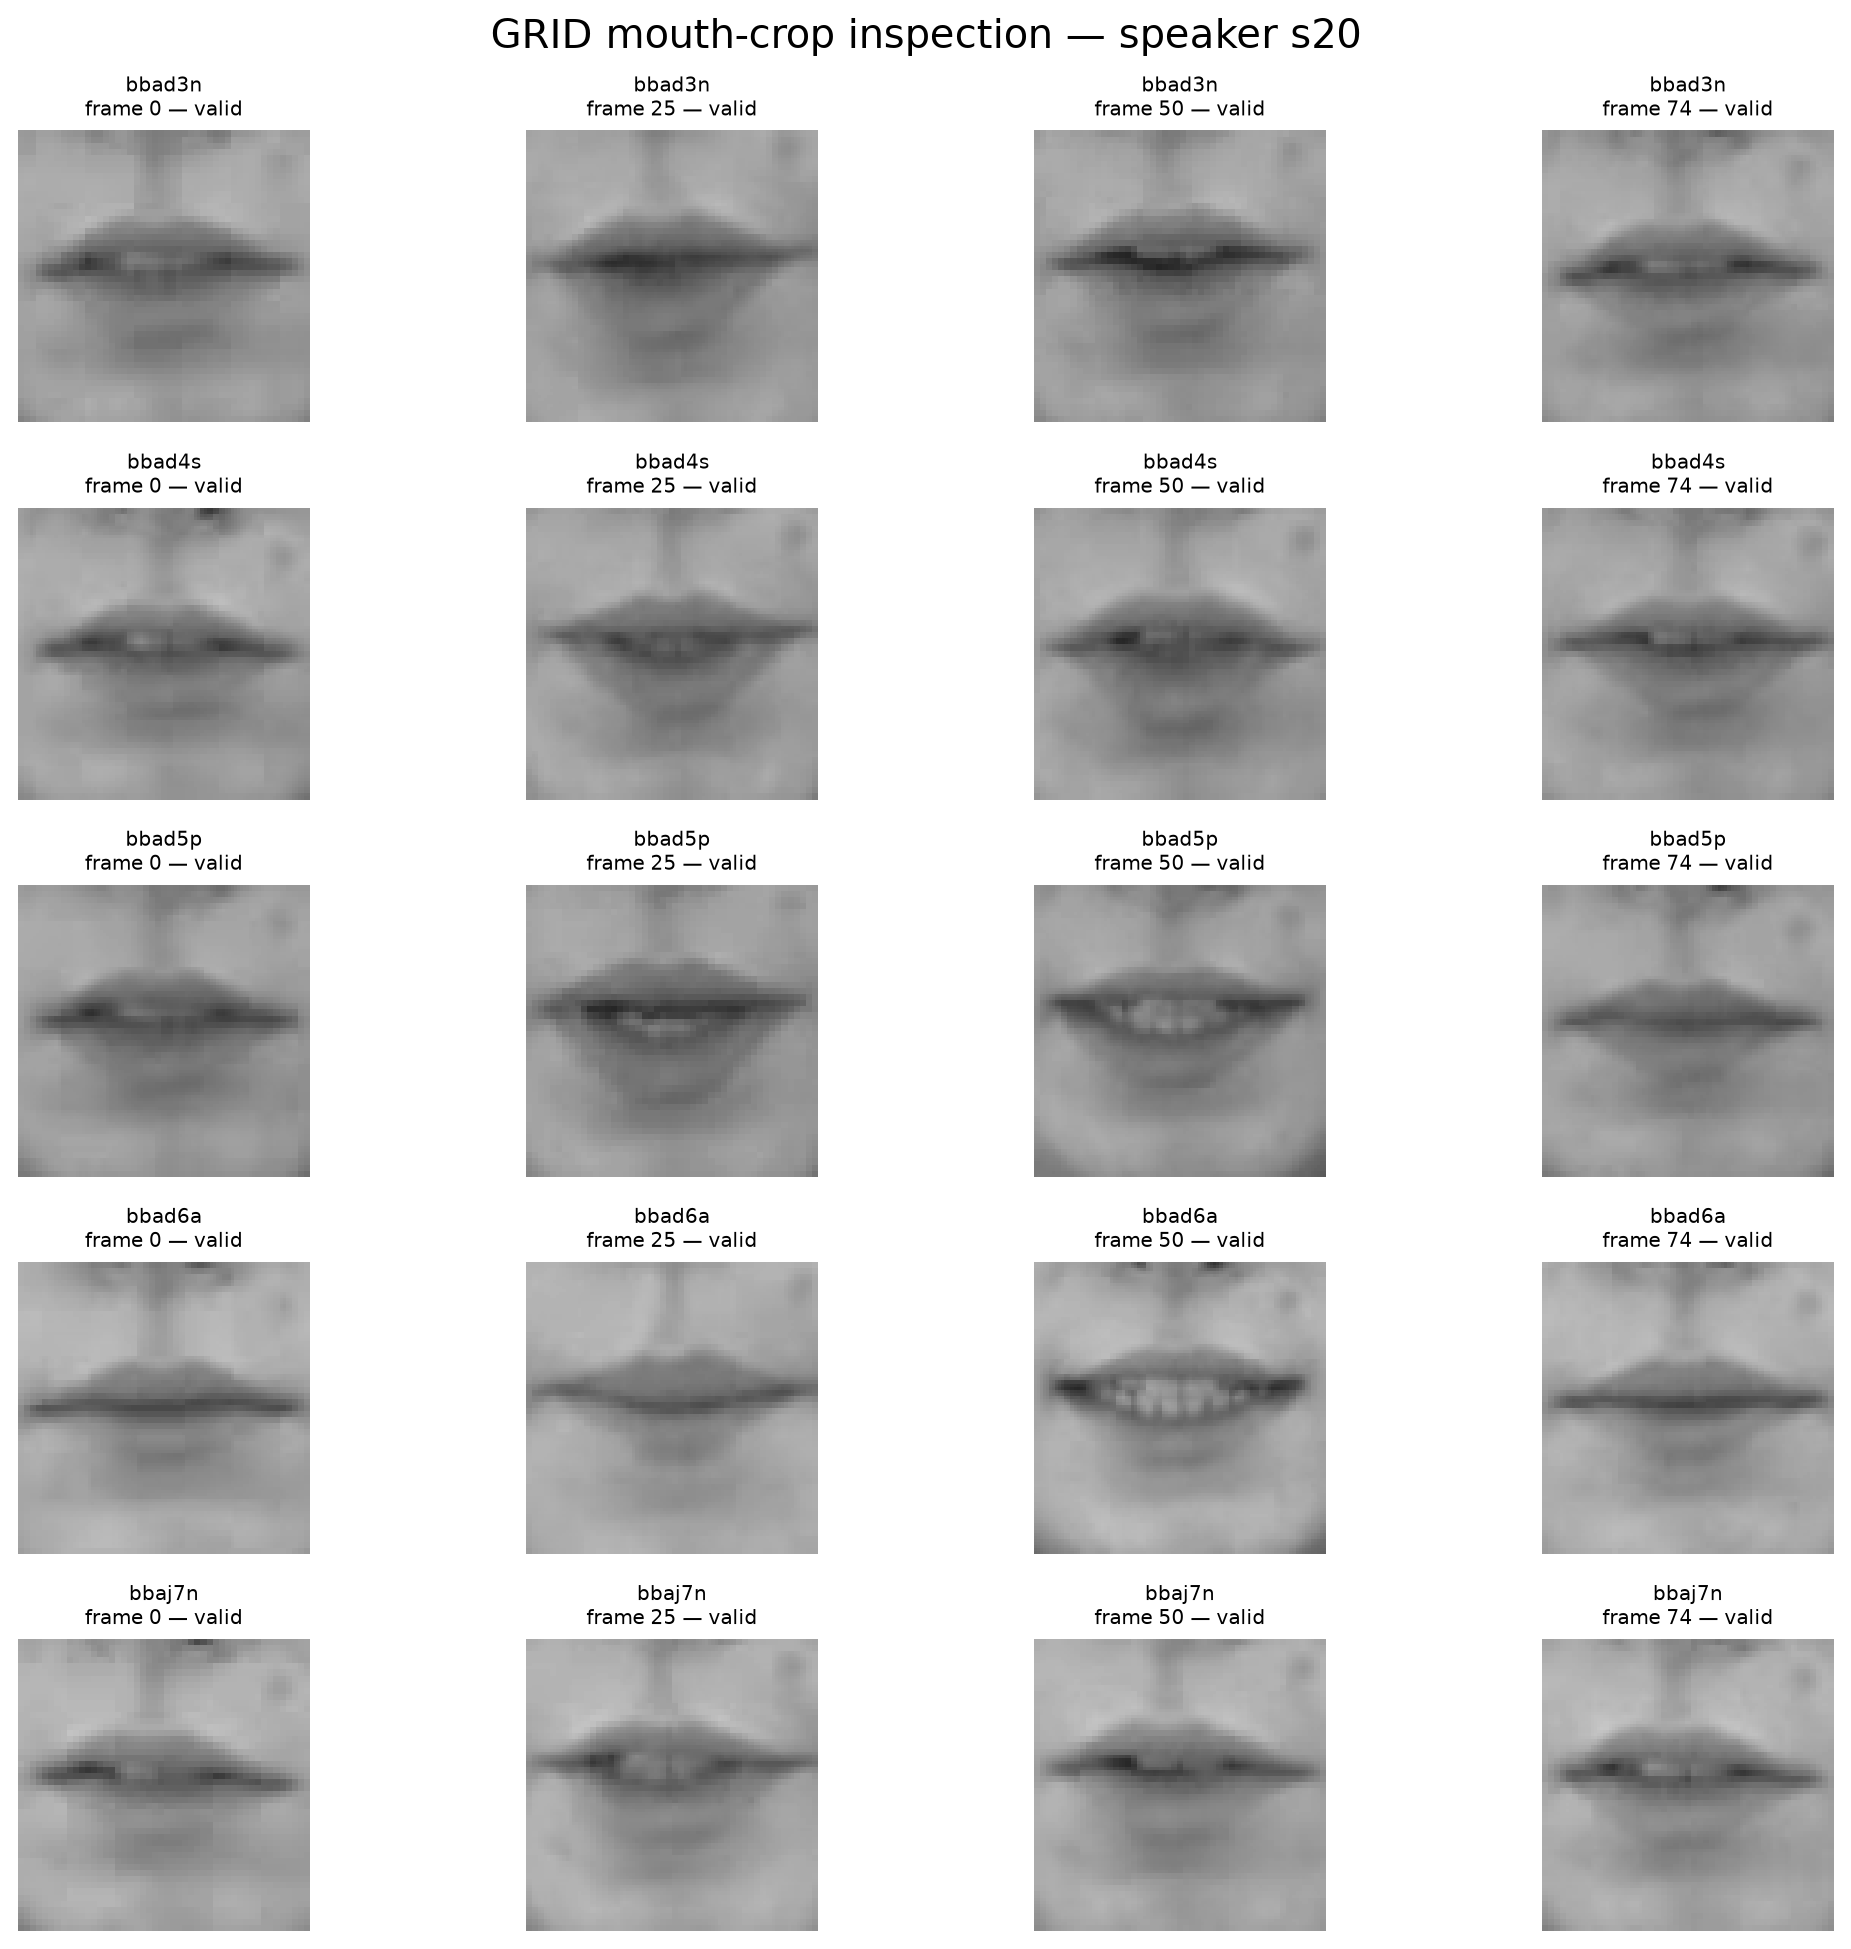
\includegraphics[width=\linewidth]{../week1 and 2 report/figures/s20_contact_sheet.png}
\end{minipage}\hfill
\begin{minipage}[t]{0.64\textwidth}\vspace{0pt}
  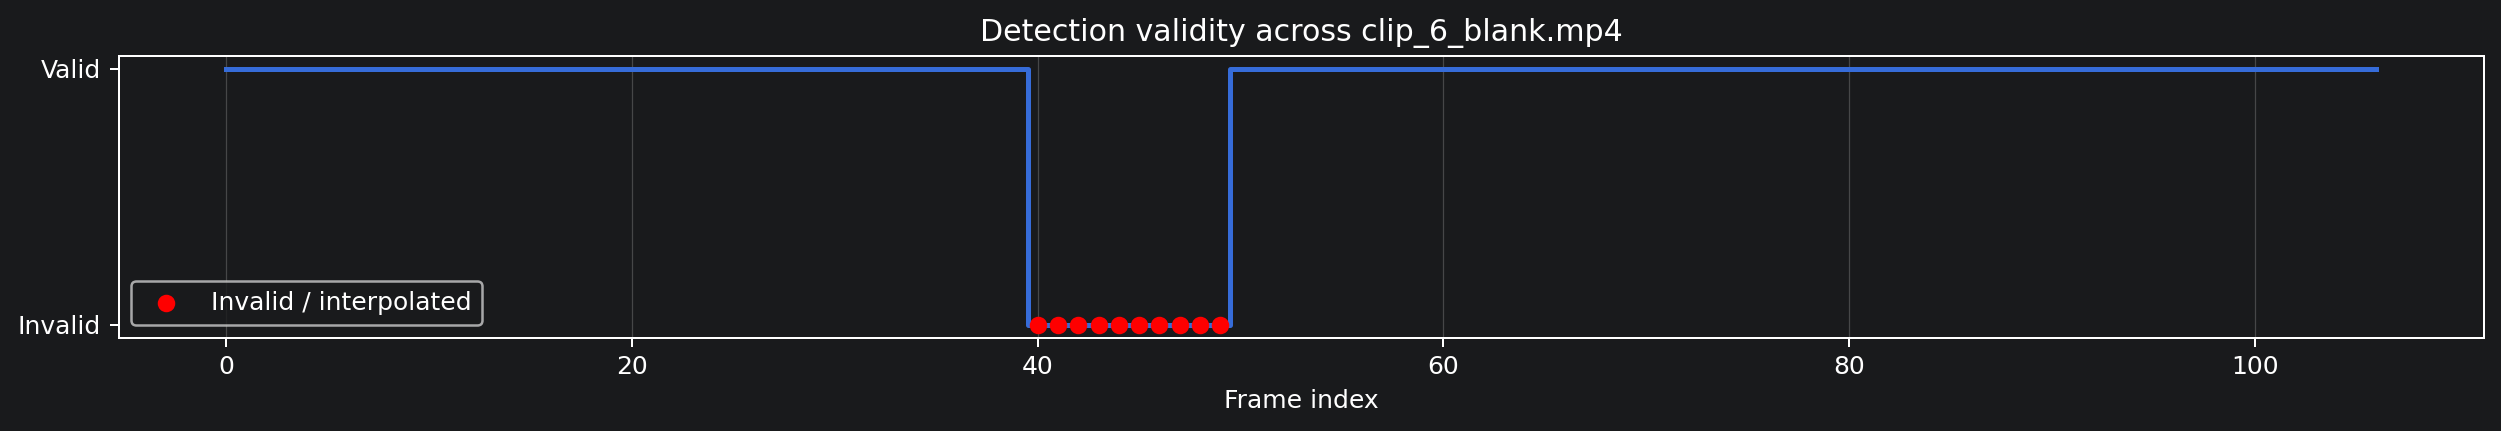
\includegraphics[width=\linewidth]{../../../docs/mouth_crop/clip_6_blank_validity.png}
  \captionof{figure}{\textbf{Left:} Contact sheet for speaker \code{s20} (frames 0, 25, 50, 74 across 5 clips), centred and stable. \textbf{Above:} Failure-handling verification on a clip with frames 40--49 artificially blanked out---the crop box is smoothly interpolated from neighbouring frames and marked invalid without dropping a single frame.}
  \label{fig:crops_handbook}
\end{minipage}
\end{figure}

\begin{lstlisting}[language=bash,caption={Week 1--2 Data Verification, Mouth Extraction, and Audio Preparation Commands}]
# 1. Audit all 34,000 GRID utterances and write reports/integrity_report.csv:
.venv/bin/python -m scripts.verify_dataset

# 2. Extract 96x96 mouth crops in parallel across CPU cores (resumable):
.venv/bin/python -m scripts.extract_mouths --workers 8

# 3. Standardise audio to 16 kHz mono WAV & generate fixed noisy val/test sets:
.venv/bin/python -m scripts.prepare_audio
.venv/bin/python -m scripts.make_noisy_test

# 4. Build master manifest.csv and training-only feature_norm.npz stats:
.venv/bin/python -m scripts.build_manifest
.venv/bin/python -m scripts.compute_norm_stats
\end{lstlisting}

% =====================================================================
\section{Chapter 3 --- Week 2: The 5 Integration Bugs Caught Before Training}

Every individual module passed its unit tests in isolation, but when Charis and I wired the end-to-end training loop together in Week~2, we uncovered and fixed \textbf{five critical integration bugs}:
\begin{enumerate}
  \item \textbf{Setback \#4 (Alignment Parser Reading Timestamps Instead of Words):} GRID \code{.align} lines have the format \code{start\_time end\_time word}. An early parser indexed token \code{0} instead of token \code{2}, turning transcripts into numbers. Fixed in \code{lipscribe/data/tokenizer.py} and verified on all 33,000 files.
  \item \textbf{Setback \#5 (End-Pointed Audio Offset):} Fixed by shifting trimmed audio waveforms according to the \code{.align} speech-start timestamp (PR~\#21).
  \item \textbf{Setback \#6 (DataLoader Workers Cloning SNR Sequences):} When PyTorch forked \code{num\_workers} processes, every worker inherited the exact same NumPy/Python RNG seed and sampled identical noise SNRs. Fixed by reseeding each worker per epoch via \code{seed + epoch * 1000 + worker\_id} (PR~\#21).
  \item \textbf{Setback \#7 (Loudness Varying with SNR):} Level-normalising to $-25\,\text{dBFS}$ \emph{before} adding noise made $-5\,\text{dB}$ clips much louder than clean clips. Moved $-25\,\text{dBFS}$ RMS normalisation (gain capped at $+20\,\text{dB}$) to run \emph{after} noise mixing (PR~\#21).
  \item \textbf{Setback \#8 (\code{.gitignore} Hiding \code{lipscribe/models/}):} An unanchored \code{models/} rule in \code{.gitignore} (meant for top-level MediaPipe weights) hid \code{lipscribe/models/} from Git. Anchored to \code{/models/}.
\end{enumerate}

% =====================================================================
\section{Chapter 4 --- Week 3 (Part 1): Baselines B1 \& B2 and the ``\code{bin blue at f sive snon}'' Overfit Mystery}

\subsection{Baseline B1: Audio-Only (\code{configs/b1\_audio\_only.yaml})}
Charis trained \textbf{B1} (\code{AudioEncoder} + \code{CTCHead}, $3.55\,\text{M}$ parameters) for \textbf{52 epochs} (best Epoch~43, $\approx 76.5\,\text{s/epoch}$ on our RTX 4080 SUPER).
\begin{itemize}
  \item \textbf{Official Held-Out Test WER:} \textbf{1.96\,\% (clean)}, $3.02\,\%$ ($10\,\text{dB}$), $3.79\,\%$ ($5\,\text{dB}$), $5.44\,\%$ ($0\,\text{dB}$), and \textbf{9.45\,\% ($-5\,\text{dB}$)}.
  \item \textbf{Takeaway:} B1 is excellent in quiet conditions ($1.96\,\%$), but its word error rate increases nearly \textbf{5-fold} at $-5\,\text{dB}$.
\end{itemize}

\subsection{Setback \#9: The B2 Visual-Only Overfit Mystery (``\code{bin blue at f sive snon}'')}
Before launching a multi-hour full-corpus visual-only run (\textbf{B2}, Card \textbf{W3-05}), our protocol required overfitting 8 utterances to $\text{CTC Loss} < 0.05$ and $\text{CER} < 0.10$. Across our first 6 runs in \code{scripts/check\_b2\_overfit.py}, the model refused to converge! Here is what we discovered:
\begin{enumerate}
  \item \textbf{Runs 1--2 (Synthetic Gaussian White Noise Collapse):} Passing \code{torch.randn} tensors through three stages of 3D convolution, BatchNorm, and MaxPool acted as a spatial low-pass filter. Feature vectors from 8 independent random clips had \textbf{87\,\% cosine similarity}, trapping CTC loss at $\approx 1.21$.
  \item \textbf{Runs 3--6 (The ``\code{bin blue at f sive snon}'' Prefix Mode Collapse):} When we loaded the first 8 real clips sequentially (\code{ds[0]..ds[7]}), the loss froze at \textbf{0.5940} and CER stuck at exactly \textbf{0.2804}. Printing the predictions revealed that the network output the exact same string for all 8 clips:
\begin{lstlisting}
[0] Ref: 'bin blue at f two now'      -> Hyp: 'bin blue at f sive snon'
[1] Ref: 'bin blue at f three soon'   -> Hyp: 'bin blue at f sive snon'
[2] Ref: 'bin blue at f four please'  -> Hyp: 'bin blue at f sive snon'
[3] Ref: 'bin blue at f five again'   -> Hyp: 'bin blue at f sive snon'
[4] Ref: 'bin blue at l six now'      -> Hyp: 'bin blue at f sive snon'
\end{lstlisting}
  \textbf{Why?} Because \code{manifest.csv} is sorted alphabetically (\code{bbaf2n}, \code{bbaf3s}...), the first 8 clips all shared the 14-character prefix \code{"bin blue at f "}! The BiLSTM memorised the shared prefix without using the 3D-CNN at all, and for the differing suffixes (\code{two/three/four/five/six/seven} + \code{now/soon/please/again}), it predicted the character-level centroid average \code{"sive snon"}---which matches $71.96\,\%$ of characters ($1 - 0.7196 = 0.2804$ CER), trapping the gradients in a deep local minimum!
  \item \textbf{Runs 7--9 (The Fix --- Unigram-Diverse Sampling \& Phase Transition):} We modified \code{load\_overfit\_batch()} to sample 8 clips with distinct starting verbs (\code{bin}, \code{lay}, \code{place}, \code{set}) and colours (\code{blue}, \code{green}, \code{red}, \code{white}). With zero shared prefix, the 3D-CNN was forced to learn real lip shapes from frame~1. At step~2,860, a phase transition occurred and loss plunged from $0.76 \to \mathbf{0.0497}$ with \textbf{CER $= 0.0000$ (100\,\% exact character match across all 8 clips)}!
\end{enumerate}

\subsection{Full-Corpus B2 Visual-Only (V1 \code{conv3d\_bilstm}) \& Setback \#10}
Full-corpus \textbf{B2 v1} trained for 28 epochs (best Epoch~19) and achieved \textbf{23.04\,\% greedy test WER} ($14.03\,\%$ CER; \textbf{21.03\,\%} with grammar decoding) across all five SNRs.
\begin{itemize}
  \item \textbf{Setback \#10 (2.5$\times$ Unseen Speaker Gap):} Per-speaker test WER varied from $13.3\,\%$ (\code{s24}) to $33.7\,\%$ (\code{s9}). Why? Because V1's three plain \code{Conv3d} blocks flatten a $96{\times}6{\times}6 = 3{,}456$ map into a dense \code{Linear(3456, 512)} layer ($1.77\,\text{M}$ params), tying weights to rigid $(x,y)$ pixel coordinates and overfitting to training speaker face geometry and lighting.
\end{itemize}

\begin{figure}[H]
\centering
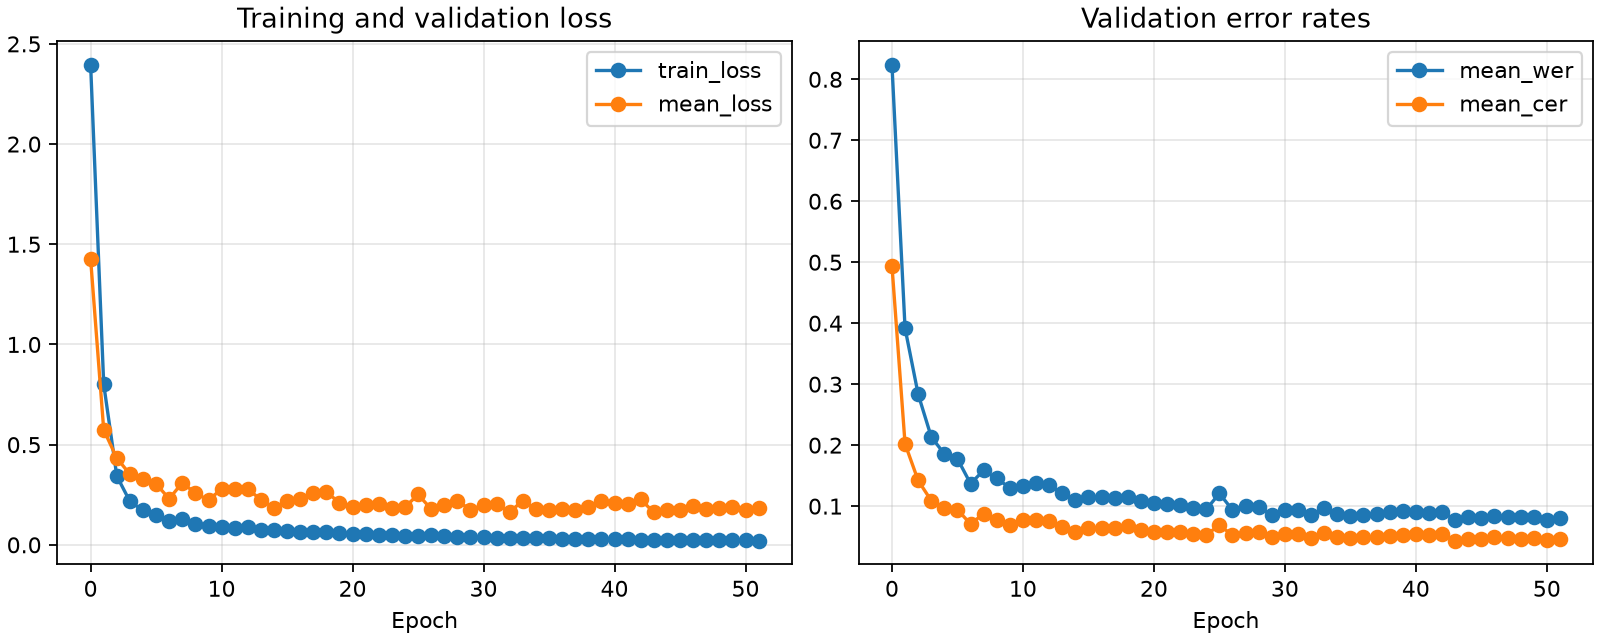
\includegraphics[width=0.48\textwidth]{../../../reports/b1_audio_only_20261103-193743/training_curves.png}\hfill
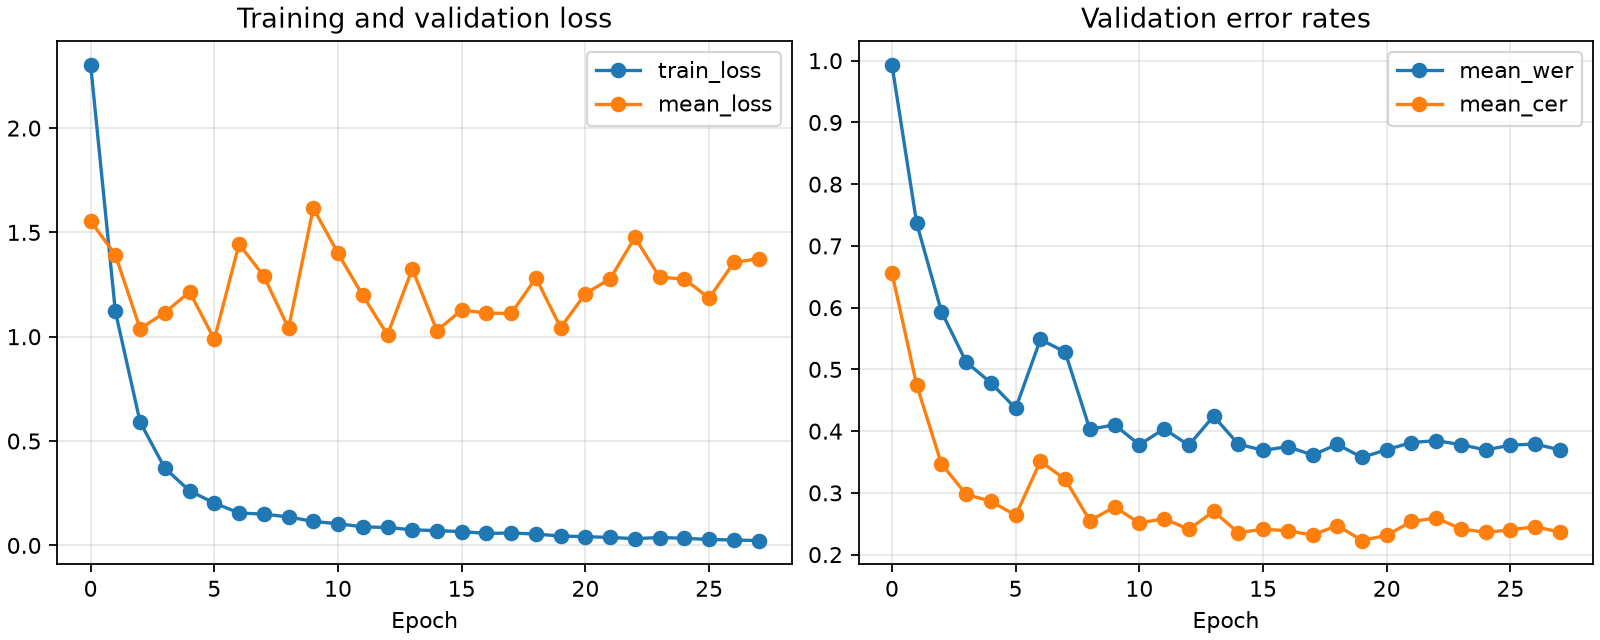
\includegraphics[width=0.48\textwidth]{../../../reports/b2_visual_only_20261104-162358/training_curves.png}
\caption{\textbf{Left:} B1 Audio-Only training and validation curves (52 epochs). \textbf{Right:} B2 Visual-Only V1 training and validation curves (28 epochs).}
\label{fig:b1_b2_curves}
\end{figure}

% =====================================================================
\section{Chapter 5 --- Week 3 (Part 2): Baseline B3, V2 Upgrades (\code{ResNet-18}), and Grammar Decoding}

\subsection{Setback \#11: Why B3 v1 (Trained From Scratch) Helped in Noise But Hurt Clean Audio}
Faith implemented \code{B3Concat} (\code{lipscribe/models/fusion\_concat.py}), which concatenates $[\mathbf{a}_t; \mathbf{v}_t] \in \mathbb{R}^{1024}$ and projects to $256$-d. When trained from scratch for 22 epochs (\textbf{B3 v1}):
\begin{itemize}
  \item At $-5\,\text{dB}$, B3 v1 beat B1 ($7.35\,\%$ vs.\ $9.45\,\%$ WER --- a $22.2\,\%$ relative reduction).
  \item \textbf{Setback \#11:} On \textbf{clean audio}, B3 v1 ($2.41\,\%$) was slightly \emph{worse} than audio-only B1 ($1.96\,\%$). Because the audio encoder converges in $\sim 10$ epochs while the visual encoder needs $25+$ epochs from scratch, the undertrained visual branch injected noise into clean audio predictions while the dominant audio gradients starved the visual encoder.
\end{itemize}

\subsection{The Four V2 Upgrades That Solved Setbacks \#10 and \#11}
\begin{enumerate}
  \item \textbf{V2 Hybrid 3D-Stem + 2D ResNet-18 Visual Encoder (\code{resnet18\_bilstm}):}
    \begin{itemize}
      \item \textbf{Per-clip photometric normalisation (\code{input\_norm="clip"}):} Standardises each clip across its valid frames to zero mean and unit variance before the first convolution, eliminating per-speaker lighting and contrast bias.
      \item \textbf{5-frame 3D spatiotemporal stem (\code{Conv3d} $5{\times}7{\times}7$):} Captures $200\,\text{ms}$ co-articulatory lip motion at the input without 3D FLOP explosion in deeper layers.
      \item \textbf{16-layer 2D ResNet-18 residual trunk + \code{AdaptiveAvgPool2d(1)}:} Replaces the coordinate-tied $3{,}456{\to}512$ flatten bottleneck with deep residual blocks and global spatial pooling, enforcing translation invariance.
      \item \textbf{Stronger augmentation:} Scale jitter ($\pm 10\,\%$), spatial cutout, time masking (two masks up to 6 frames), and \code{Dropout2d(0.2)}.
    \end{itemize}
  \item \textbf{Pre-trained Encoder Initialisation (\code{init\_from}):} Initialise multimodal models directly from the converged \code{B1} and \code{B2} checkpoints.
  \item \textbf{Modality Dropout:} Randomly zero out the audio stream ($p_a$) or visual stream ($p_v$) per training utterance so the fusion layer must learn from both modalities.
  \item \textbf{Exact GRID Grammar Viterbi Decoder (\code{lipscribe/decoding/grammar.py}):} Alongside Isabelle's CTC Prefix Beam Search ($17.29\,\text{ms/utt}$), we built a vectorised Viterbi decoder over the exact $64{,}000$-sentence GRID grammar trie ($11.0\,\text{ms/utt}$ on CPU, zero retraining required).
\end{enumerate}

\textbf{Result in B3 v2:} Initialising from \code{B1 + B2 v2} with modality dropout cut B3 v2's greedy test WER to \textbf{1.16\,\% (clean)} and \textbf{5.21\,\% ($-5\,\text{dB}$)}---\textbf{0.77\,\% (clean)} and \textbf{3.83\,\% ($-5\,\text{dB}$)} with grammar decoding!
\begin{itemize}
  \item \textbf{Setback \#12 (B3 v2's Fatal Unimodal Collapse):} When we tested B3 v2 with one modality removed at test time (\code{--drop-modality visual} or \code{--drop-modality audio}), B3 v2 collapsed to \textbf{25.18\,\% WER without video} and \textbf{75.31\,\% WER without audio} because linear concatenation has no dynamic gate or learned missing-modality representation.
\end{itemize}

% =====================================================================
\section{Chapter 6 --- Week 4: Proposed Model P (Cross-Modal Attention, Gated Fusion, \code{e\_miss}, and Full Results)}

\subsection{How Proposed Model P (\code{LipScribeModel}) Works}
Implemented in \code{lipscribe/models/fusion\_attention.py} (Cards \textbf{W4-01} to \textbf{W4-04}), \textbf{Model~P} introduces three mechanisms that solve B3's limitations:
\begin{enumerate}
  \item \textbf{Learned Missing-Modality Embedding ($\mathbf{e}_{\text{miss}} \in \mathbb{R}^{256}$):}
    \emph{Setback \#12b:} If you mask all keys in \code{nn.MultiheadAttention} when a stream is missing, $\text{softmax}(-\infty,\dots,-\infty)$ produces \code{NaN}! Instead, whenever a stream is dropped (during training modality dropout $p_a=0.25, p_v=0.15$, test-time \code{--drop-modality}, or live inference when MediaPipe detects a face in $< 50\,\%$ of frames), we replace that stream's projected features with the learned vector $\mathbf{e}_{\text{miss}}$.
  \item \textbf{Bidirectional 4-Head Cross-Modal Attention (\code{CrossModalAttention}):}
    Audio queries Video ($\tilde{\mathbf{a}} = \text{LN}(\mathbf{a}_{\text{proj}} + \text{MHA}(Q=\mathbf{a}_{\text{proj}}, K=\mathbf{v}_{\text{proj}}, V=\mathbf{v}_{\text{proj}}))$) and Video queries Audio ($\tilde{\mathbf{v}} = \text{LN}(\mathbf{v}_{\text{proj}} + \text{MHA}(Q=\mathbf{v}_{\text{proj}}, K=\mathbf{a}_{\text{proj}}, V=\mathbf{a}_{\text{proj}}))$).
  \item \textbf{Per-Frame Sigmoid Gated Fusion (\code{GatedFusion}):}
    $$\mathbf{g}_t = \sigma\!\left(\mathbf{W}_g [\tilde{\mathbf{a}}_t; \tilde{\mathbf{v}}_t] + \mathbf{b}_g\right) \in (0, 1)^{256}, \qquad \mathbf{f}_t = \mathbf{g}_t \odot \tilde{\mathbf{a}}_t + (1 - \mathbf{g}_t) \odot \tilde{\mathbf{v}}_t$$
\end{enumerate}

\subsection{Full-Corpus 4-Way Model P Experiment (\code{P1}, \code{P2}, \code{P3}, \code{P4})}
We trained all four initialisation variants of Model~P on the \textbf{full GRID corpus} (30-minute wall-clock budget per variant on the RTX 4080 SUPER, matching B3 v2):
\begin{itemize}
  \item \textbf{P1 (\code{p\_scratch}):} Audio and visual (\code{Conv3D}) trained from scratch (11 epochs).
  \item \textbf{P2 (\code{p\_init\_b2}):} Visual initialised from \code{B2 v1} (\code{Conv3D}); audio random (11 epochs).
  \item \textbf{P3 (\code{p\_init\_b1\_b2}):} Audio from \code{B1} + visual from \code{B2 v1} (\code{Conv3D}) (10 epochs).
  \item \textbf{P4 (\code{p\_init\_b1\_b2\_v2} / \code{p\_proposed}):} Audio from \code{B1} + visual from \code{B2 v2} (\code{ResNet-18}) (6 epochs).
\end{itemize}

\begin{figure}[H]
\centering
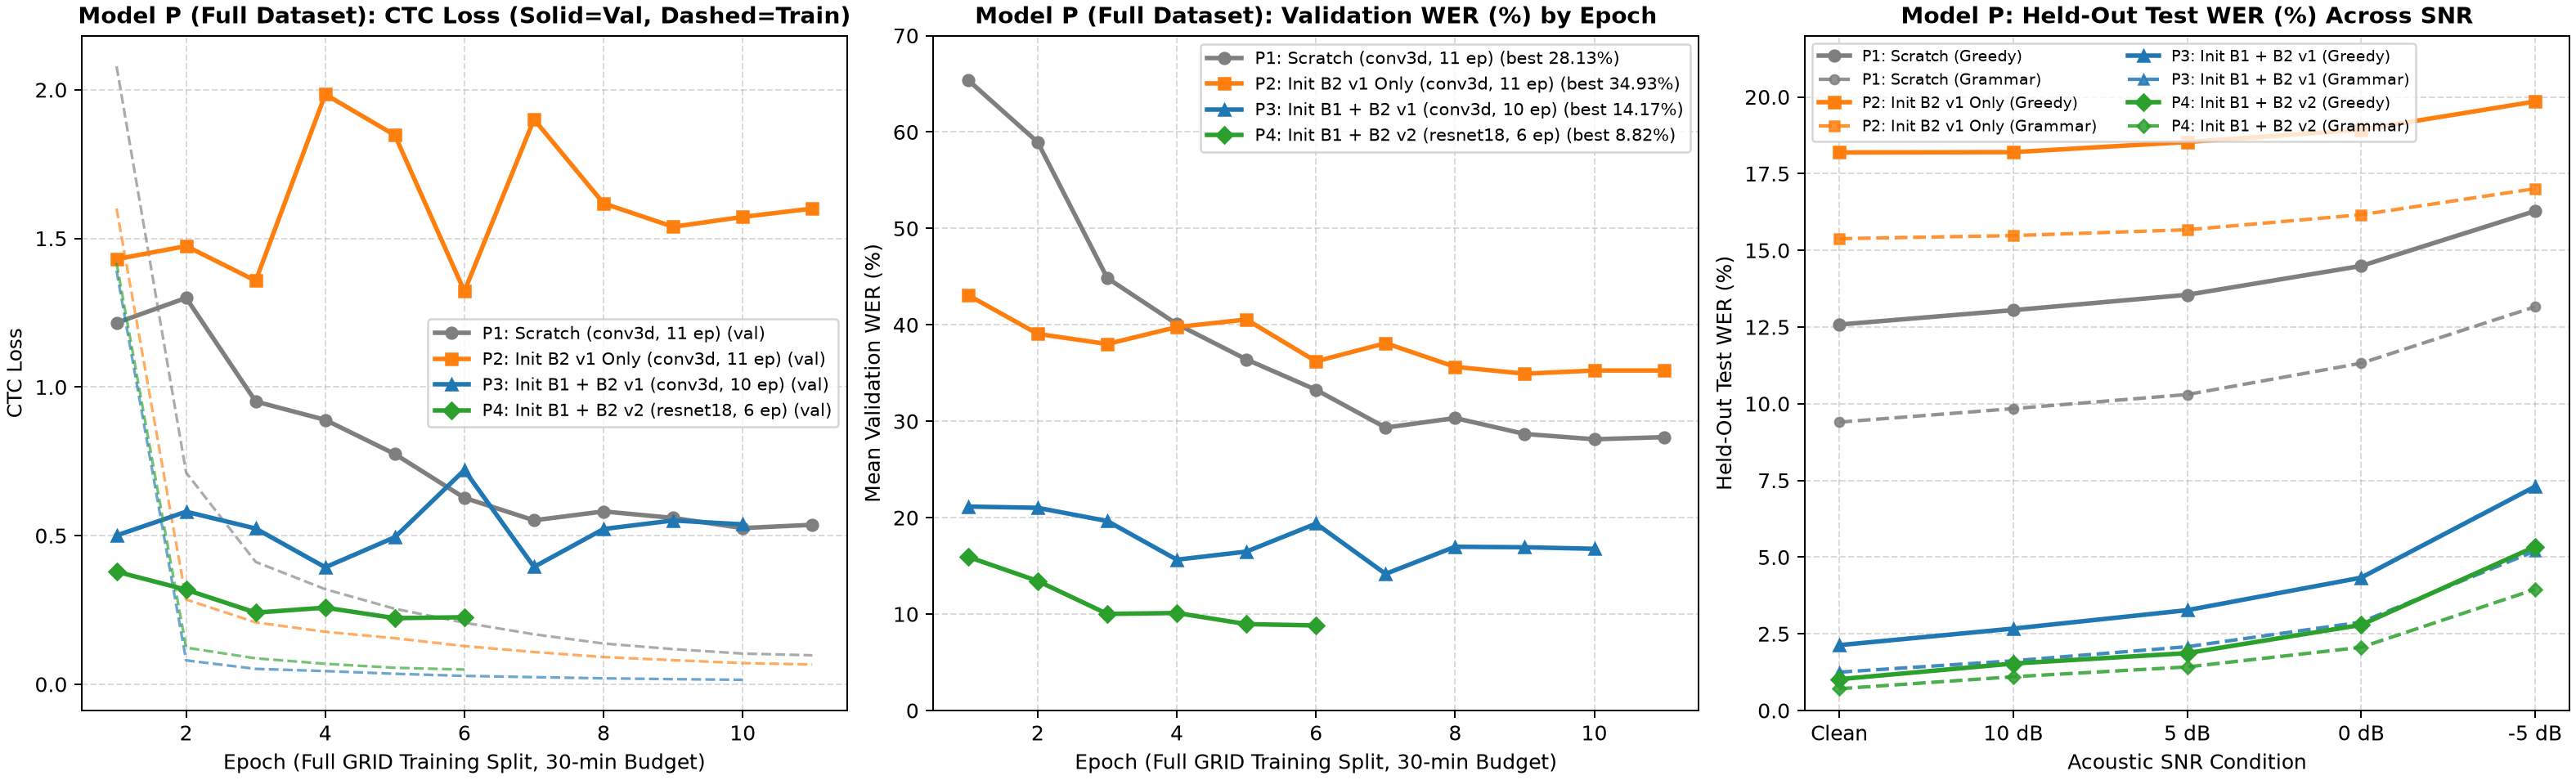
\includegraphics[width=\textwidth]{../../../reports/model_p_4way_curriculum.png}
\caption{Full-corpus 4-way Model P comparison (\code{P1--P4}): CTC loss convergence (left), validation WER trajectory by epoch (centre), and official held-out test WER across all 5 SNRs for greedy and grammar decoding (right).}
\label{fig:p_4way}
\end{figure}

\begin{figure}[H]
\centering
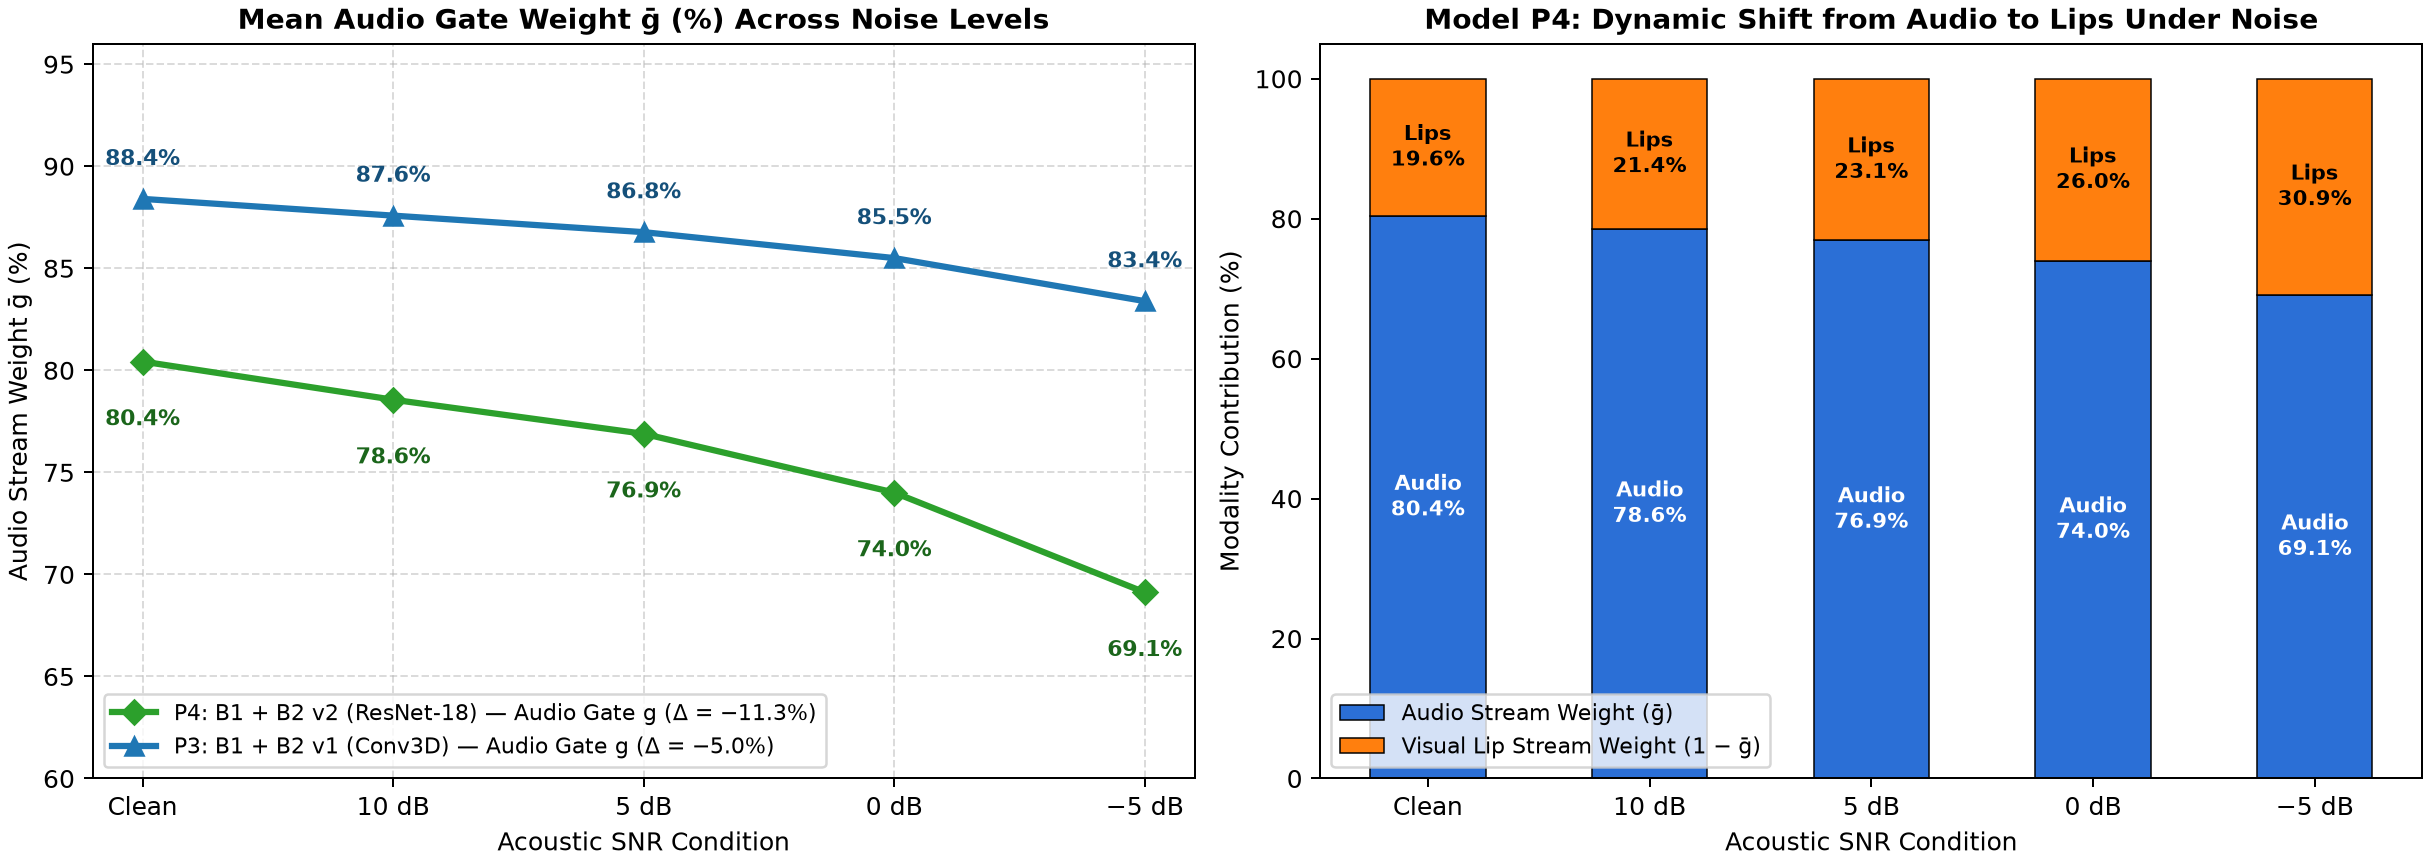
\includegraphics[width=\textwidth]{../../../reports/model_p_gate_vs_snr.png}
\caption{\textbf{Proof of Dynamic Noise-Adaptive Gating:} As acoustic noise increases from Clean to $-5\,\text{dB}$, Model P4 monotonically lowers its audio gate $\bar{g}$ from $80.4\,\%$ down to $69.1\,\%$ ($\Delta\bar{g} = -11.3\,\%$, $2.25\times$ stronger than P3's \code{Conv3D} gate shift), increasing visual lip reliance from $19.6\,\%$ up to $30.9\,\%$.}
\label{fig:gate_vs_snr}
\end{figure}

% =====================================================================
\section{Chapter 7 --- Master Scoreboard \& Complete Log of All 13 Setbacks}

\begin{figure}[H]
\centering
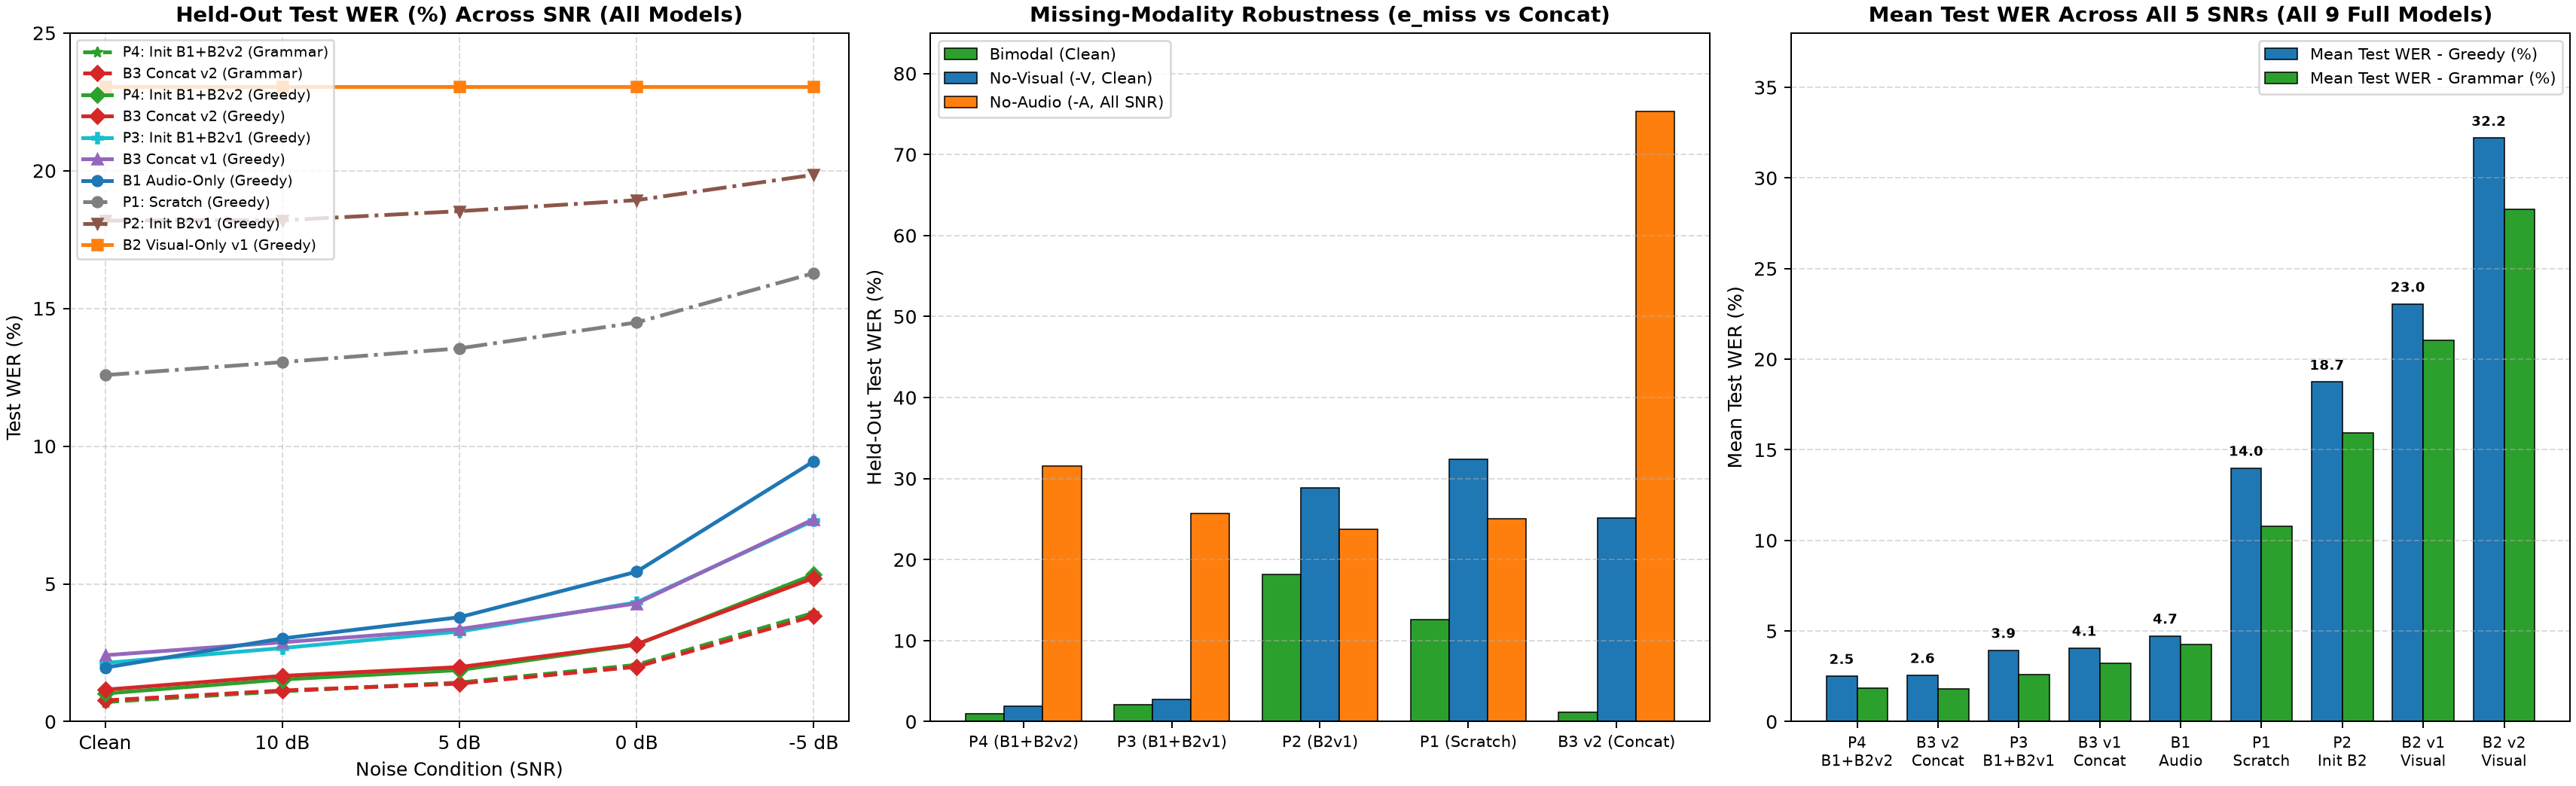
\includegraphics[width=\textwidth]{../../../reports/all_models_snr_and_summary.png}
\caption{Master comparison across all 9 full-corpus models: Held-out test WER vs.\ SNR (left), missing-modality robustness comparing $\mathbf{e}_{\text{miss}}$ against concatenation (centre), and mean test WER across all 5 SNRs (right).}
\label{fig:all_models}
\end{figure}

\begin{table}[H]
\centering
\caption{Master Scoreboard: Official Held-Out Test WER \% Across All 9 Full-Corpus Trained Models (3,998 test utterances per SNR).}
\label{tab:master_scoreboard}
\resizebox{\textwidth}{!}{%
\rowcolors{2}{lsrow}{white}
\begin{tabular}{@{}llccccccccc@{}}
\toprule
\rowcolor{white}\sffamily\bfseries Model & \sffamily\bfseries Visual / Init & \textbf{Val WER} & \textbf{Clean Grd/Grm} & \textbf{10\,dB Grd/Grm} & \textbf{5\,dB Grd/Grm} & \textbf{0\,dB Grd/Grm} & \textbf{$-$5\,dB Grd/Grm} & \textbf{Mean Grd/Grm} & \textbf{No-Aud ($-$A)} & \textbf{No-Vis ($-$V Cln)} \\
\midrule
\textbf{B1 Audio-Only} & --- / Scratch & 7.72 & 1.96 / 1.76 & 3.02 / 2.79 & 3.79 / 3.47 & 5.44 / 4.93 & 9.45 / 8.35 & 4.73 / 4.26 & --- & 1.96 \\
\textbf{B2 Visual v1} & \code{Conv3D} / Scr & 35.74 & 23.04 / 21.03 & 23.04 / 21.03 & 23.04 / 21.03 & 23.04 / 21.03 & 23.04 / 21.03 & 23.04 / 21.03 & 23.04 & --- \\
\textbf{B2 Visual v2} & \code{Res18} / Scr & 42.38 & 32.20 / 28.26 & 32.20 / 28.26 & 32.20 / 28.26 & 32.20 / 28.26 & 32.20 / 28.26 & 32.20 / 28.26 & 32.20 & --- \\
\textbf{B3 Concat v1} & \code{Conv3D} / Scr & 12.37 & 2.41 / 1.86 & 2.88 / 2.27 & 3.36 / 2.65 & 4.29 / 3.45 & 7.35 / 5.87 & 4.06 / 3.22 & --- & --- \\
\textbf{B3 Concat v2} & \code{Res18} / B1+B2v2 & 8.72 & 1.16 / 0.77 & 1.66 / 1.13 & 1.98 / \textbf{1.38} & 2.81 / \textbf{1.99} & \textbf{5.21 / 3.83} & 2.56 / \textbf{1.82} & 75.31 & 25.18 \\
\textbf{Model P1} & \code{Conv3D} / Scr & 28.13 & 12.58 / 9.40 & 13.05 / 9.84 & 13.55 / 10.30 & 14.49 / 11.32 & 16.28 / 13.16 & 13.99 / 10.80 & 25.03 & 32.41 \\
\textbf{Model P2} & \code{Conv3D} / B2v1 & 34.93 & 18.19 / 15.38 & 18.20 / 15.48 & 18.53 / 15.67 & 18.93 / 16.16 & 19.85 / 17.01 & 18.74 / 15.94 & \textbf{23.78} & 28.82 \\
\textbf{Model P3} & \code{Conv3D} / B1+B2v1 & 14.17 & 2.13 / 1.25 & 2.67 / 1.62 & 3.27 / 2.08 & 4.33 / 2.88 & 7.30 / 5.20 & 3.94 / 2.61 & 25.65 & 2.72 \\
\textbf{Model P4 (Best)} & \code{Res18} / B1+B2v2 & \textbf{8.82} & \textbf{1.02 / 0.71} & \textbf{1.53 / 1.10} & \textbf{1.87} / 1.42 & \textbf{2.79} / 2.06 & 5.34 / 3.95 & \textbf{2.51} / 1.85 & 31.57 & \textbf{1.88} \\
\bottomrule
\end{tabular}%
}
\end{table}

\begin{table}[H]
\centering\scriptsize
\caption{Complete Chronological Log of All 13 Setbacks Encountered and Engineering Solutions Taken.}
\label{tab:setbacks}
\rowcolors{2}{lsrow}{white}
\begin{tabularx}{\textwidth}{@{}cL{1.8cm}L{3.8cm}L{3.9cm}X@{}}
\toprule
\rowcolor{white}\sffamily\bfseries \# & \sffamily\bfseries Stage & \sffamily\bfseries Setback Encountered & \sffamily\bfseries Root Cause & \sffamily\bfseries Solution Implemented \\
\midrule
1 & W1-07 Audit & Speaker \code{s21} missing video; $110$ corrupt clips in \code{s8}, \code{s4}, \code{s28} & Raw GRID archive defects & Built \code{verify\_dataset.py} to exclude \code{s21} and filter bad clips ($32{,}890$ valid kept) \\
2 & W1-07 Sync & Audio lasted $1.1\text{--}2.9\,\text{s}$ vs.\ $3.0\,\text{s}$ video; voice $\sim 0.47\,\text{s}$ early & GRID \code{.wav} files were end-pointed (silence trimmed) & Shifted audio placement in \code{GridDataset} using \code{.align} word-onset timestamps \\
3 & W2-01 Crop & MediaPipe missed faces on 1--2 frames in some clips & Brief motion blur or extreme lip posture & Linearly interpolated boxes from neighbour frames and marked \code{valid[t]=False} (kept $T=75$) \\
4 & W2-09 Align & Early transcripts decoded as numbers instead of words & \code{.align} parser read column \code{0} (time) instead of \code{2} (word) & Fixed \code{parse\_align()} in \code{tokenizer.py}; verified on all $33{,}000$ files \\
5 & W2-09 RNG & DataLoader workers drew identical SNR sequences & Forked workers inherited identical RNG state & Reseeded RNG deterministically per \code{(seed, epoch, worker\_id)} \\
6 & W2-07 RMS & $-5\,\text{dB}$ mixtures were much louder than clean clips & $-25\,\text{dBFS}$ levelling ran \emph{before} noise mixing & Moved RMS normalisation to run \emph{after} noise mixing (gain $\le +20\,\text{dB}$) \\
7 & W2-11 Git & \code{lipscribe/models/} files hidden from \code{git status} & Unanchored \code{models/} rule in \code{.gitignore} & Anchored rule to \code{/models/} in \code{.gitignore} \\
8 & W3-05 Overfit & B2 overfit froze at $\text{CER}=0.2804$, predicting \code{'bin blue at f sive snon'} & First 8 alphabetical clips shared \code{'bin blue at f '}; BiLSTM predicted suffix centroid & Sampled unigram-diverse verbs/colours (\code{load\_overfit\_batch}), hitting $\text{Loss}=0.0497, \text{CER}=0.0$ \\
9 & W3-05 B2 v1 & $2.5\times$ WER gap across unseen speakers ($13.3\,\%$ vs.\ $33.7\,\%$) & Shallow 3-block \code{Conv3d} + \code{Linear(3456,512)} overfit to speaker geometry & Built \code{ResNetVisualEncoder} (\code{resnet18\_bilstm}) with \code{input\_norm="clip"} and \code{AdaptiveAvgPool2d(1)} \\
10 & W3-06 B3 v1 & B3 v1 beat B1 at $-5\,\text{dB}$ ($7.35\,\%$) but hurt clean speech ($2.41\,\%$ vs.\ $1.96\,\%$) & Fast-converging audio starved slow random-init visual stream & Added pre-trained checkpoint loading (\code{init\_from}) + modality dropout $\to$ $1.16\,\%$ clean in B3 v2 \\
11 & W4-pre Ablat. & Dropping video or audio collapsed B3 v2 ($25.18\,\%$ / $75.31\,\%$) & Fixed linear concatenation lacks dynamic gating or fallback token & Built \textbf{Model P} with learned $\mathbf{e}_{\text{miss}}$, cross-attention, and gate $\mathbf{g}_t$ ($1.88\,\%$ no-video, $23.78\,\%$ no-audio) \\
12 & W4-02 Mask & Masking all keys in \code{MultiheadAttention} gave \code{NaN} & $\text{softmax}(-\infty,\dots,-\infty) = \text{NaN}$ & Substituted learned $\mathbf{e}_{\text{miss}} \in \mathbb{R}^{256}$ \emph{before} attention instead of masking all keys \\
13 & W4-04 Eval & \code{evaluate.py} crashed with \code{ValueError: 'gate\_mean'} on Model P & \code{save\_metrics()} had fixed 5-column header without \code{gate\_mean} & Updated \code{save\_metrics()} in \code{scripts/evaluate.py} to include \code{gate\_mean} dynamically \\
\bottomrule
\end{tabularx}
\end{table}

% =====================================================================
\section{Chapter 8 --- Team Command Cheat-Sheet: Run Everything Yourself}

\begin{lstlisting}[language=bash,caption={Complete Command Reference (Run from Repo Root on the Alienware Workstation)}]
# 1. Run the complete unit & integration test suite (pytest):
.venv/bin/python -m pytest -q

# 2. Run 8-utterance overfit sanity checks (< 2 minutes each):
.venv/bin/python -m scripts.check_b2_overfit
.venv/bin/python -m scripts.check_b3_overfit
.venv/bin/python -m scripts.check_p_overfit

# 3. Train any Baseline or Proposed Model P variant (inside tmux):
tmux new -s lipscribe
.venv/bin/python -m scripts.train --config configs/b1_audio_only.yaml
.venv/bin/python -m scripts.train --config configs/b2_visual_only.yaml
.venv/bin/python -m scripts.train --config configs/b3_concat_v2.yaml --time-budget-min 30
.venv/bin/python -m scripts.train --config configs/p_init_b1_b2_v2.yaml --time-budget-min 30

# 4. Evaluate our best Model P checkpoint (Greedy, Grammar, Beam Search, & Modality Ablations):
.venv/bin/python -m scripts.evaluate --checkpoint checkpoints/p_proposed_best.pt
.venv/bin/python -m scripts.evaluate --checkpoint checkpoints/p_proposed_best.pt --decode grammar
.venv/bin/python -m scripts.evaluate --checkpoint checkpoints/p_proposed_best.pt --decode beam
.venv/bin/python -m scripts.evaluate --checkpoint checkpoints/p_proposed_best.pt --drop-modality audio
.venv/bin/python -m scripts.evaluate --checkpoint checkpoints/p_proposed_best.pt --drop-modality visual

# 5. Regenerate all comparison plots and report figures:
.venv/bin/python -m scripts.plot_all_model_comparisons
\end{lstlisting}

\end{document}
